\begin{figure}[h]
	\centering
	\setlength{\imgWidth}{1.55in}
	\addtolength{\tabcolsep}{-3.5pt}
	\begin{tabular}{cccc}
		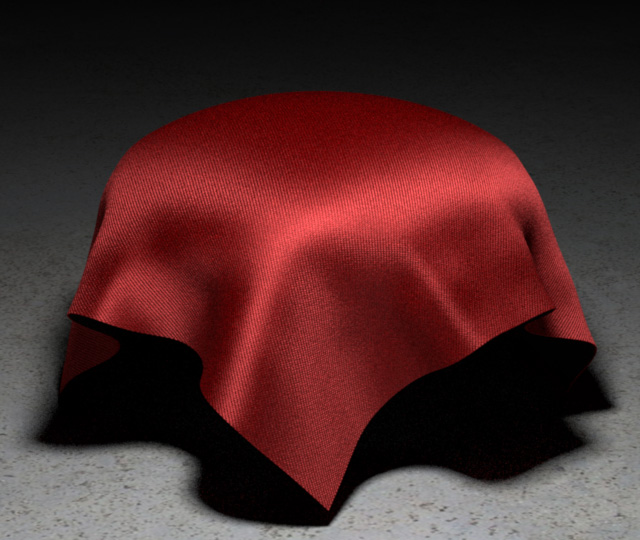
\includegraphics[width=\imgWidth]{layeredbsdf/results/gabardine_ref.jpg} &
		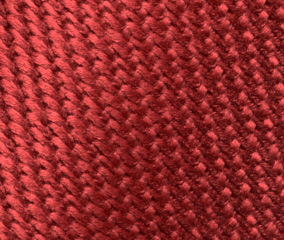
\includegraphics[width=\imgWidth]{layeredbsdf/results/gabardine_ref_inset_128spp.jpg} &
		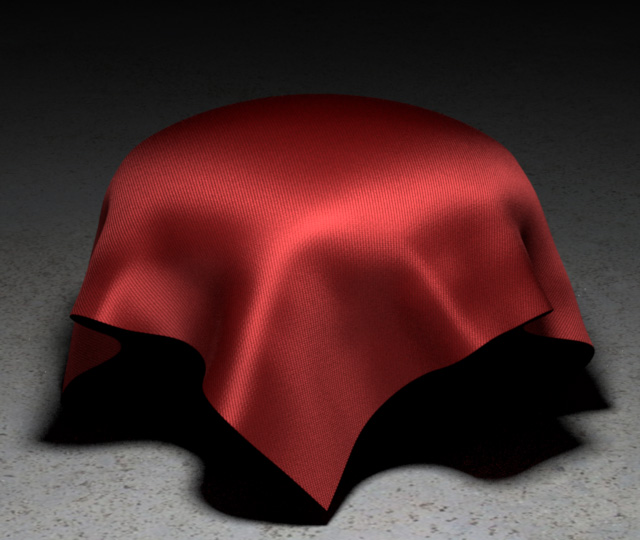
\includegraphics[width=\imgWidth]{layeredbsdf/results/gabardine.jpg} &
		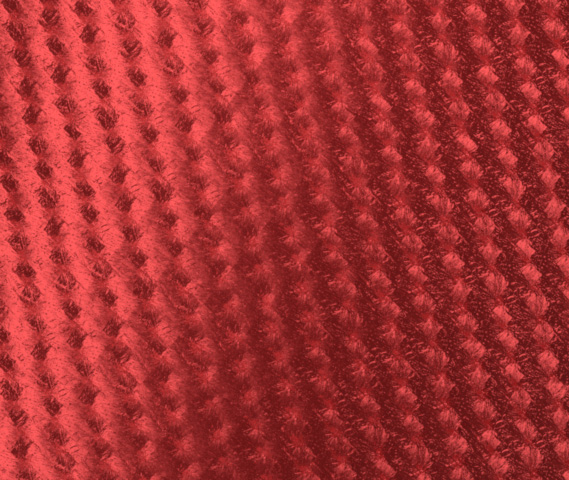
\includegraphics[width=\imgWidth]{layeredbsdf/results/gabardine_inset_512spp.jpg} \\
		\multicolumn{2}{c}{(a) Volume rendering} & \multicolumn{2}{c}{(b) Our BSDF + fiber-direction map}
	\end{tabular}
	\caption[Comparison to volumetric cloth]{\label{fig:layeredbsdf:cloth_compare}
		\textbf{Comparison to volumetric cloth.} \textbf{(a)} Images rendered from micro-CT volumetric data, using the microflake phase function. \textbf{(b)} Renderings using our approach using a single microflake volumetric layer, where we are using fiber direction maps extracted from the volumetric data. Our rendering is 40$\times$ faster than the volumetric simulation.
	}
\end{figure} 